%\begin{frame}{PCA examples}{example 1}
    %\begin{columns}
    %\column{.5\linewidth}
        %\begin{itemize}
            %\item 4-dimensional feature space: Spectral Centroid, RMS, Zero Crossing, Spectral Rolloff
            %\item 10 classes of music signals (classical, jazz, blues, metal, ...)
        %\end{itemize}
    %\column{.4\linewidth}
        %\figwithmatlab{FeatureScatter}
    %\end{columns}
%\end{frame}

\begin{frame}{PCA examples}{example 1: scatter and classification}
		\vspace{-8mm}
    \begin{columns}
    \column{.5\linewidth}
        \begin{itemize}
            \item 4-dimensional feature space: 
							\begin{itemize}
									\item	Spectral Centroid $\mu_\mathrm{SC}$
									\item RMS $\mu_\mathrm{RMS}$
									\item Zero Crossing $\mu_\mathrm{ZC}$
									\item Spectral Rolloff $\mu_\mathrm{SR}$
							\end{itemize}
						\smallskip
            \item 10 classes of music signals 
							\begin{itemize}
								\item blues
								\item classical
								\item country
								\item disco
								\item hiphop
								\item jazz
								\item metal
								\item	pop
								\item reggae
								\item rock
							\end{itemize}
        \end{itemize}
    \column{.5\linewidth}
        \only<1>{\figwithmatlab{FeatureScatter}}
        \only<2>{\vspace{-4mm}\figwithmatlab{FeatureScatterPca}}
    \end{columns}
\end{frame}

\begin{frame}{PCA examples}{example 1: scatter and classification}
		\vspace{-5mm}
    \begin{columns}
    \column{.5\linewidth}
        
        \begin{itemize}
            \item \textbf{experiment: feature/pc classification performance}
							\begin{itemize}
								\item individual 
								\item cumulative 
							\end{itemize}
            \bigskip
						\item<2-> \textbf{observations}
            \begin{itemize}
                \item   combined feature performance is not sum of individual performance
                \item   variance/eigenvalue ranking does not necessarily correlate to task performance
                \item   simple feature selection is not necessarily inferior to PCA
            \end{itemize}
        \end{itemize}
    \column{.4\linewidth}
        \vspace{-5mm}
        \figwithmatlab{PcaClassification}
    \end{columns}
\end{frame}

\begin{frame}{PCA examples}{example 2: feature analysis}
    \textbf{PCA transformation matrix $\mathbf{T}^\mathrm{T}$}
    \only<1>
    {
            \begin{equation}\left[ 
                    \begin{array}{cccccc} 
   -0.5638 &  -0.3596 &  -0.5024 &  -0.5481\\
    0.1738 &  -0.9139 &   0.3539 &   0.0965\\
    0.2408 &  -0.1882 &  -0.7606 &   0.5728\\
   -0.7707 &  -0.0018 &   0.2096 &   0.6017\nonumber
                     \end{array}  
            \right]         \end{equation}   }
    \only<2>{
            \begin{equation}\left[ 
                    \begin{array}{cccccc} 
   \textcolor{highlight}{-0.5638} &  -0.3596 &  \textcolor{highlight}{-0.5024} &  \textcolor{highlight}{-0.5481}\\
    0.1738 &  \textcolor{highlight}{-0.9139} &   0.3539 &   0.0965\\
    0.2408 &  -0.1882 &  \textcolor{highlight}{-0.7606} &   \textcolor{highlight}{0.5728}\\
   \textcolor{highlight}{-0.7707} &  -0.0018 &   0.2096 &   \textcolor{highlight}{0.6017}\nonumber

%\textcolor{highlight}{-0.4187} &   0.3467  & \textcolor{highlight}{-0.4569}  &  0.4143 &  -0.1271 &  \textcolor{highlight}{-0.5549}\\
%-0.3908 &   0.1815  &  \textcolor{highlight}{0.8136}  & -0.0289 &   0.2060 &  -0.3304\\
%\textcolor{highlight}{-0.4516} &   0.3384  &  0.0859  &  0.2413 &  -0.2919 &   \textcolor{highlight}{0.7285}\\
%\textcolor{highlight}{-0.4337} &   0.1699  & -0.3337  & \textcolor{highlight}{-0.7243} &   0.3747 &   0.0816\\
%0.3802 &   \textcolor{highlight}{0.5599}  & -0.0381  &  0.2808 &   \textcolor{highlight}{0.6622} &   0.1524\\
%0.3679 &   \textcolor{highlight}{0.6245}  &  0.0956  & -0.4071 &  \textcolor{highlight}{-0.5267} &  -0.1495\nonumber
                     \end{array}  
            \right]         \end{equation}   
						}
						\begin{figure}%
						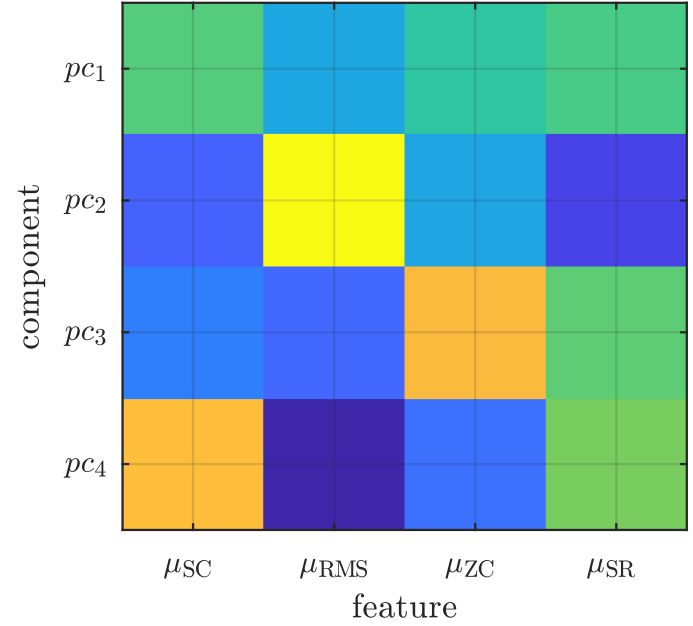
\includegraphics[width=.3
						\columnwidth]{transformation_matrix}%
						\end{figure}
    
\end{frame}
